\subsection{Definitions and Terms}
\begin{frame}
\frametitle{Definitions and Terms}

\begin{block}{Unknown Region}
A territory that has not been covered yet by the robot's sensors
\end{block}

\pause
\begin{block}{Known Region}
A territory that has already been covered by the robot's sensors
\end{block}

\pause
\begin{block}{Open-Space}
A \emph{known region} which does not contain an obstacle
\end{block}


\end{frame}

\begin{frame}
\frametitle{Definitions and Terms (cond.)}
\begin{block}{Occupied-Space}
A \emph{known region} which contains an obstacle
\end{block}

\pause

\begin{block}{Frontier}
\begin{itemize}
  \item A segment that separates \emph{known} regions from unknown regions
  \item Frontier is a set of \emph{unknown} points that each have at least one
  \emph{open-space} neighbor
\end{itemize}

\end{block}
\end{frame}

\begin{frame}
\begin{figure}
 \centering
 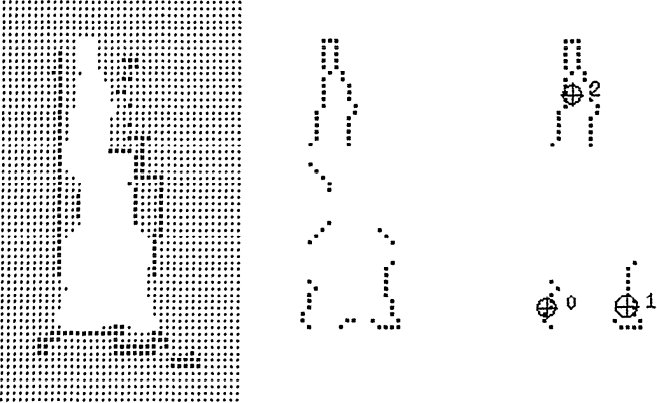
\includegraphics[width=0.8\columnwidth,keepaspectratio]{images/frontiers_example.jpg}
 \caption{Image taken from \citep{yamauchi_frontier-based_1998}: evidence
 grid, frontier points, extraction of different frontiers (from left to right).}
\end{figure}
\end{frame}